
Figure \ref{fig: l2 errors test 1} shows the $L^2$ error of all performances of the first test case that have converged, the polynomial degrees $k$ were taken to be $1,\dots,3$ and $k_{DH}$ equal to all variants $0, \dots, k$. In Figure \ref{fig: h1 errors test 1} the corresponding $H^1$ errors are plotted.
The results for the runs with $k=3$ are shown in more detail in Table \ref{tab: l2 errors test 1 deg 2}. %, again the column $N$ refers to the number of iterations the Newton solver needed to reach the desired tolerance. 

Due to the large number of degree of freedoms the requested memory for the cases $k=2,3$ and $k_{DH}=2,3$ on the finest grid, and for $k=3$ and $k_{DH}=3$ all meshes with $h\geq 1/64$ is too much. Even though matrices during Newont's method are sparse their $LU$ decomposition is in general not. Replacing the linear solver by different iterative solvers\footnote{GMRES with an algebraic multigrid preconditioner, GMRES with an incomplete $LU$ factorisation, GMRES with Jacobi preconditioning, BiCGStab with preconditioning} yielded to divergence of either the Newton or the linear solver.

\begin{figure}[H]
\centering
	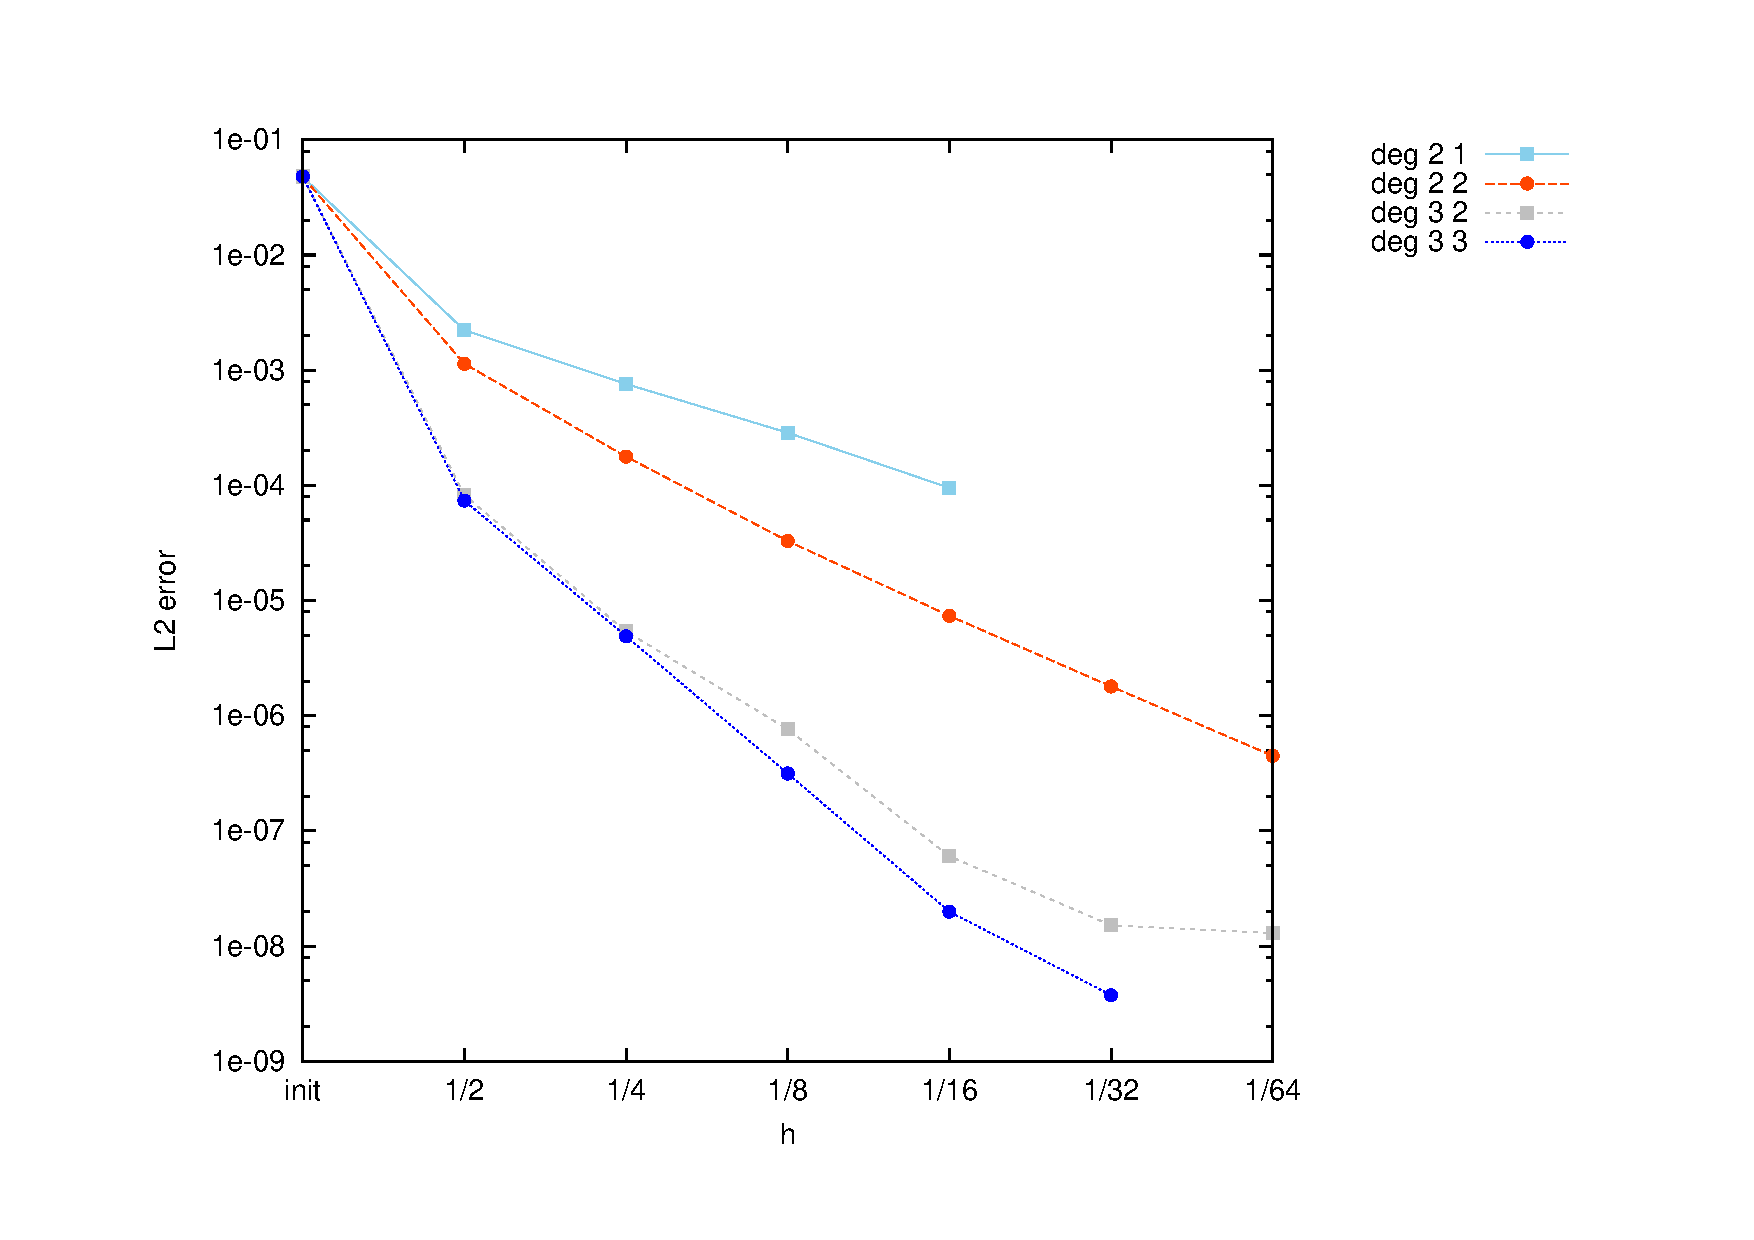
\includegraphics[scale =0.45]{plots/MA1_Neilan_l2.pdf}
	\caption{$L^2$ errors for Test \ref{test smooth}}
	\label{fig: l2 errors test 1}
\end{figure}
\begin{table}[H]
	\begin{subtable}[b]{0.45\textwidth}
		\centering
		\pgfplotstabletypeset[columns={iterations, l2error, h1error,N},
		every row 0 column 0/.style={set content=init},
		every row 6 column 1/.style={set content=-},
		every row 6 column 2/.style={set content=-},
		every row 6 column 3/.style={set content=-},
		]\MAOnedegThreeThree
		\caption{Error for $k=3, k_{DH}=3$}
	\end{subtable}
	~
	\begin{subtable}[b]{0.45\textwidth}
		\centering
		\pgfplotstabletypeset[columns={iterations, l2error, h1error,N},
		every row 0 column 0/.style={set content=init},
		]\MAOnedegThreeTwo
		\caption{Error for $k=3, k_{DH}=2$}
	\end{subtable}
	\caption{Errors for Test \ref{test smooth}}
	\label{tab: l2 errors test 1 deg 2}
\end{table}
\begin{figure}[H]
\centering
	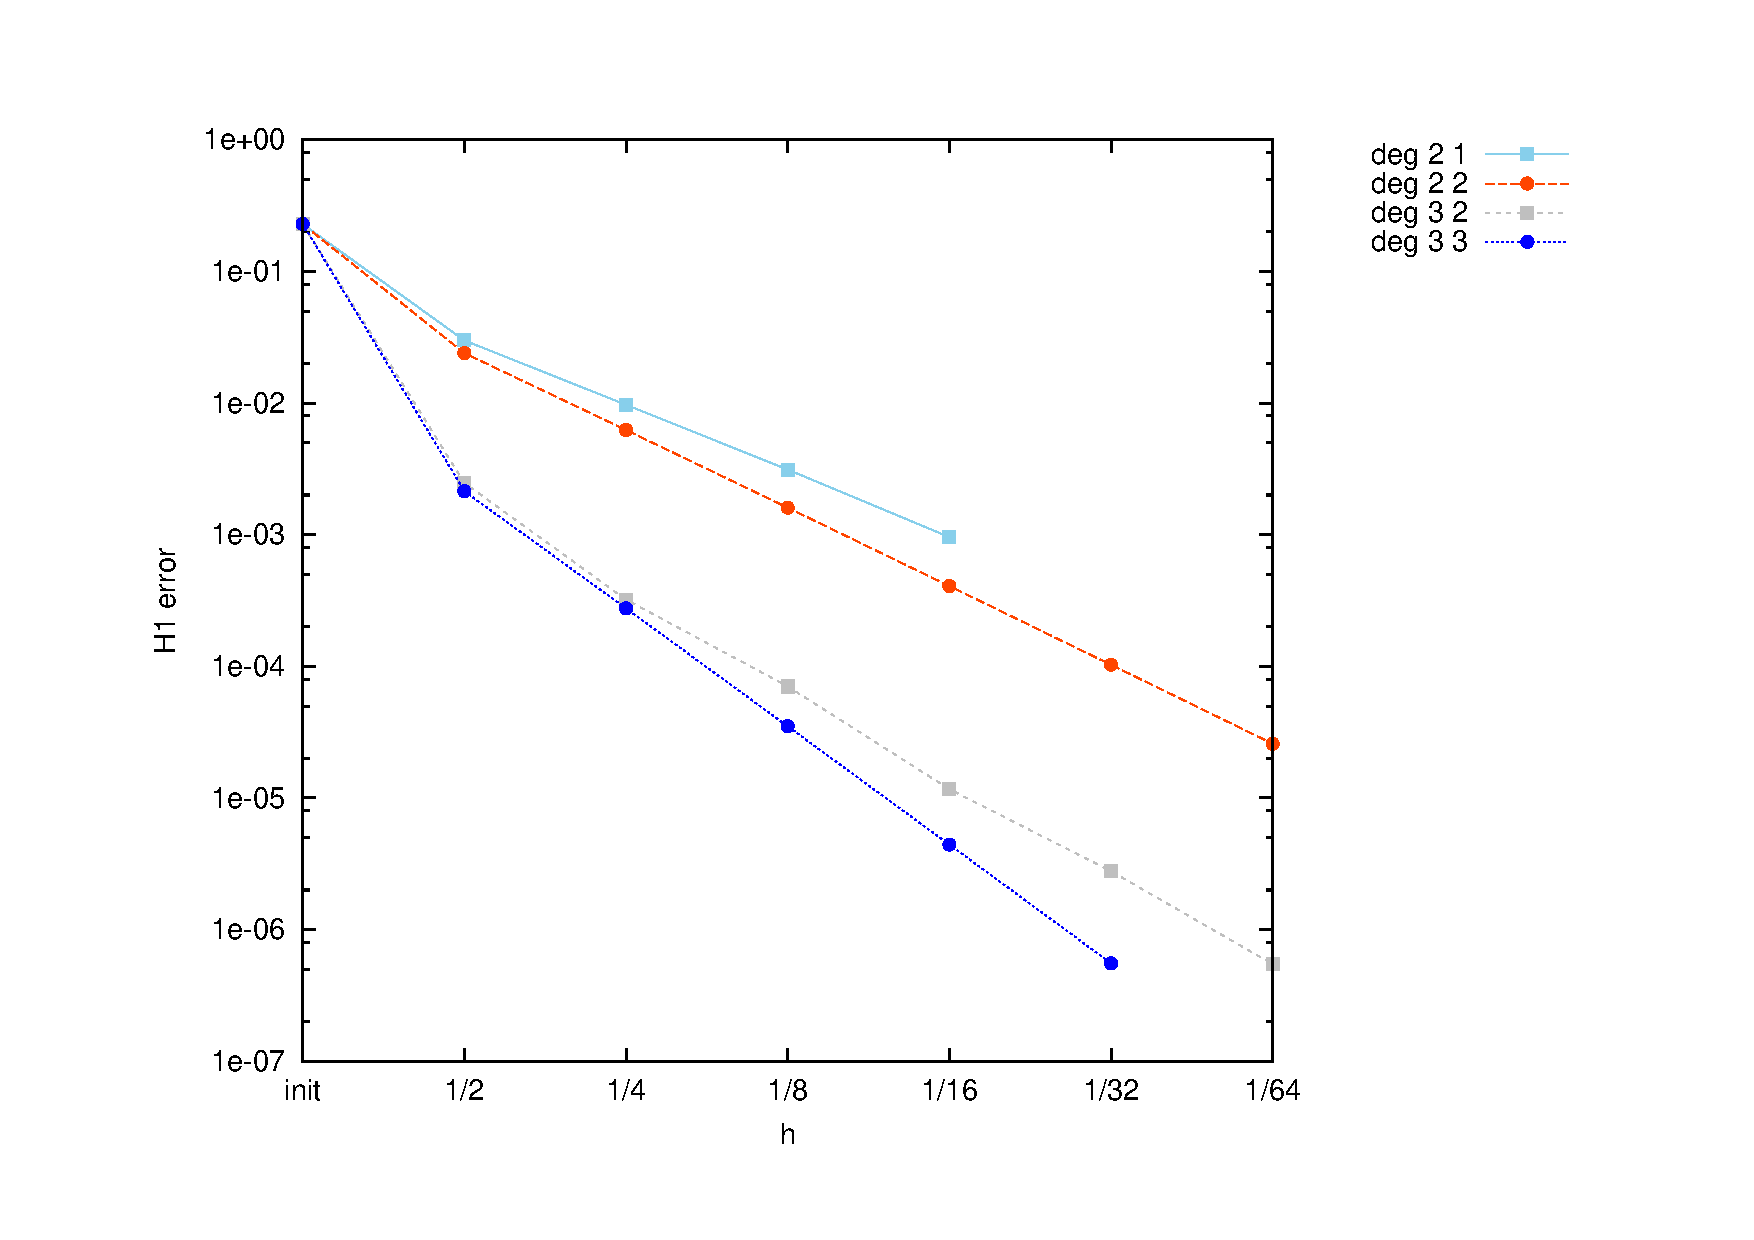
\includegraphics[scale =0.45]{plots/MA1_Neilan_h1.pdf}
	\caption{$H^1$ errors for Test \ref{test smooth}}
	\label{fig: h1 errors test 1}
\end{figure}

As also experienced by Neilan \cite{Neilan2014} the method does not converge for the polynomial degree $k=1$. Similarly, in runs with a low polynomial degree $k_{DH}$ Newton's method did not converge.
Considering these results we observe that the error almost do not alter for different polynomial degrees $k_{DH}$ if both converge. Nevertheless for fine grids the methods without difference between the two degrees seem to perform better. The calculated numerical orders as shown in Table \ref{tab: order} support this first intuition.

\begin{table}[H]
\begin{subtable}[b]{0.45\textwidth}
\centering
	\pgfplotstabletypeset
	{
		k $k_{DH}$ {numerical order}
		2 1  1.50338
		2 2  2.24427
		3 2 2.63597
		3 3 3.64758
	}
	\caption{Numerical order in $L^2$ norm}
\end{subtable}
\begin{subtable}[b]{0.45\textwidth}
	\pgfplotstabletypeset
	{
		k $k_{DH}$ {numerical order}
		2 1  1.65382 
		2 2  1.973
		3 2 2.39616
		3 3 2.97876
	}
	\caption{Numerical order in $H^1$ norm}
	\end{subtable}
\caption{Numerical order in Test \ref{test smooth}}
\label{tab: order}
\end{table}

This test scenario, i.e. Test \ref{test smooth}, has also been performed with the additional normal jump penalty term as proposed by Neilan and stated in \eqref{eq: neilan eq1 + jump} weighted with weight $\eta$. 

Fortunately, the method converges if the linear solver was set to GMRES preconditioned by an incomplete $LU$ factorisation. Thus, the nonlinear solver was adjusted to handle linear system with this iterative method. The results are shown in Figure \ref{fig: l2 errors test 1 jump}, Table \ref{tab: l2 errors test 1 deg 2 jump} and Table \ref{tab: l2 errors test 1 deg 3 jump}. 

\begin{figure}[h!]
\centering
	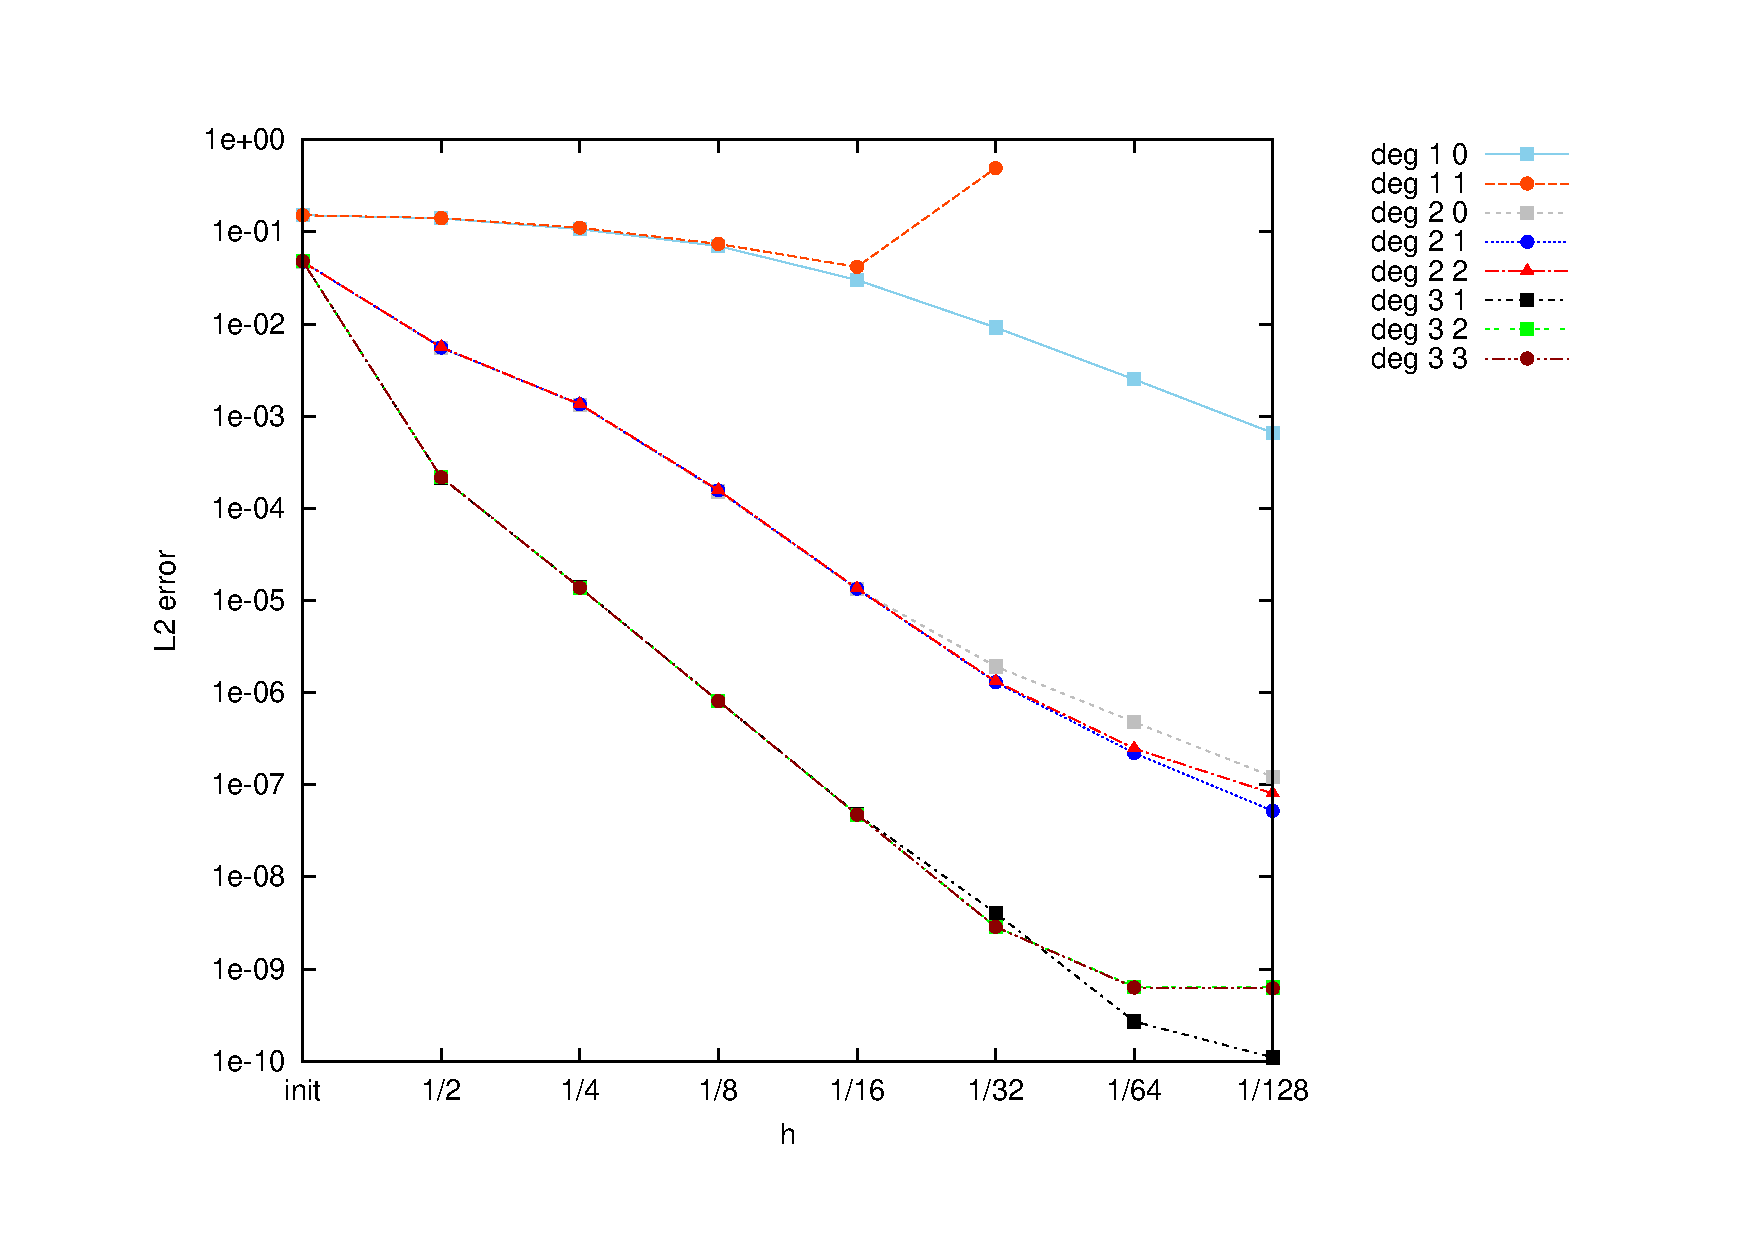
\includegraphics[scale=0.45]{plots/MA1_Neilan_GradJump_l2.pdf}
	\caption{$L^2$ errors for Test \ref{test smooth} with additional gradient jump penalty}
	\label{fig: l2 errors test 1 jump}
\end{figure}
\begin{table}[H]
	\begin{subtable}[b]{0.4\textwidth}
		\centering
		\pgfplotstabletypeset[
		columns={iterations, l2error, h1error,N},
		every row 0 column 0/.style={set content=init},
		]\MAOneJumpdegTwoTwo
		\caption{Error for $k=2, k_{DH}=2$}
	\end{subtable}
	\hspace{0.7cm}
	\begin{subtable}[b]{0.4\textwidth}
		\centering
		\pgfplotstabletypeset[columns={iterations, l2error, h1error,N},
		every row 0 column 0/.style={set content=init},
		]\MAOneJumpdegTwoZero
		\caption{Error for $k=2, k_{DH}=0$}
	\end{subtable}
	\caption{Errors for Test \ref{test smooth} with additional jump penalty}
	\label{tab: l2 errors test 1 deg 2 jump}
\end{table}
\begin{table}[h]
	\begin{subtable}[b]{0.45\textwidth}
		\centering
		\pgfplotstabletypeset[
		columns={iterations, l2error, h1error,N},
		every row 0 column 0/.style={set content=init},
		]\MAOneJumpdegThreeThree
		\caption{Error for $k=3, k_{DH}=3$}
	\end{subtable}
	~
	\begin{subtable}[b]{0.45\textwidth}
		\centering
		\pgfplotstabletypeset[columns={iterations, l2error, h1error,N},
		every row 0 column 0/.style={set content=init},
		]\MAOneJumpdegThreeTwo
		\caption{Error for $k=3, k_{DH}=2$}
	\end{subtable}
	\caption{Errors for Test \ref{test smooth} with additional jump penalty}
	\label{tab: l2 errors test 1 deg 3 jump}
\end{table}

\begin{figure}[H]
\centering
	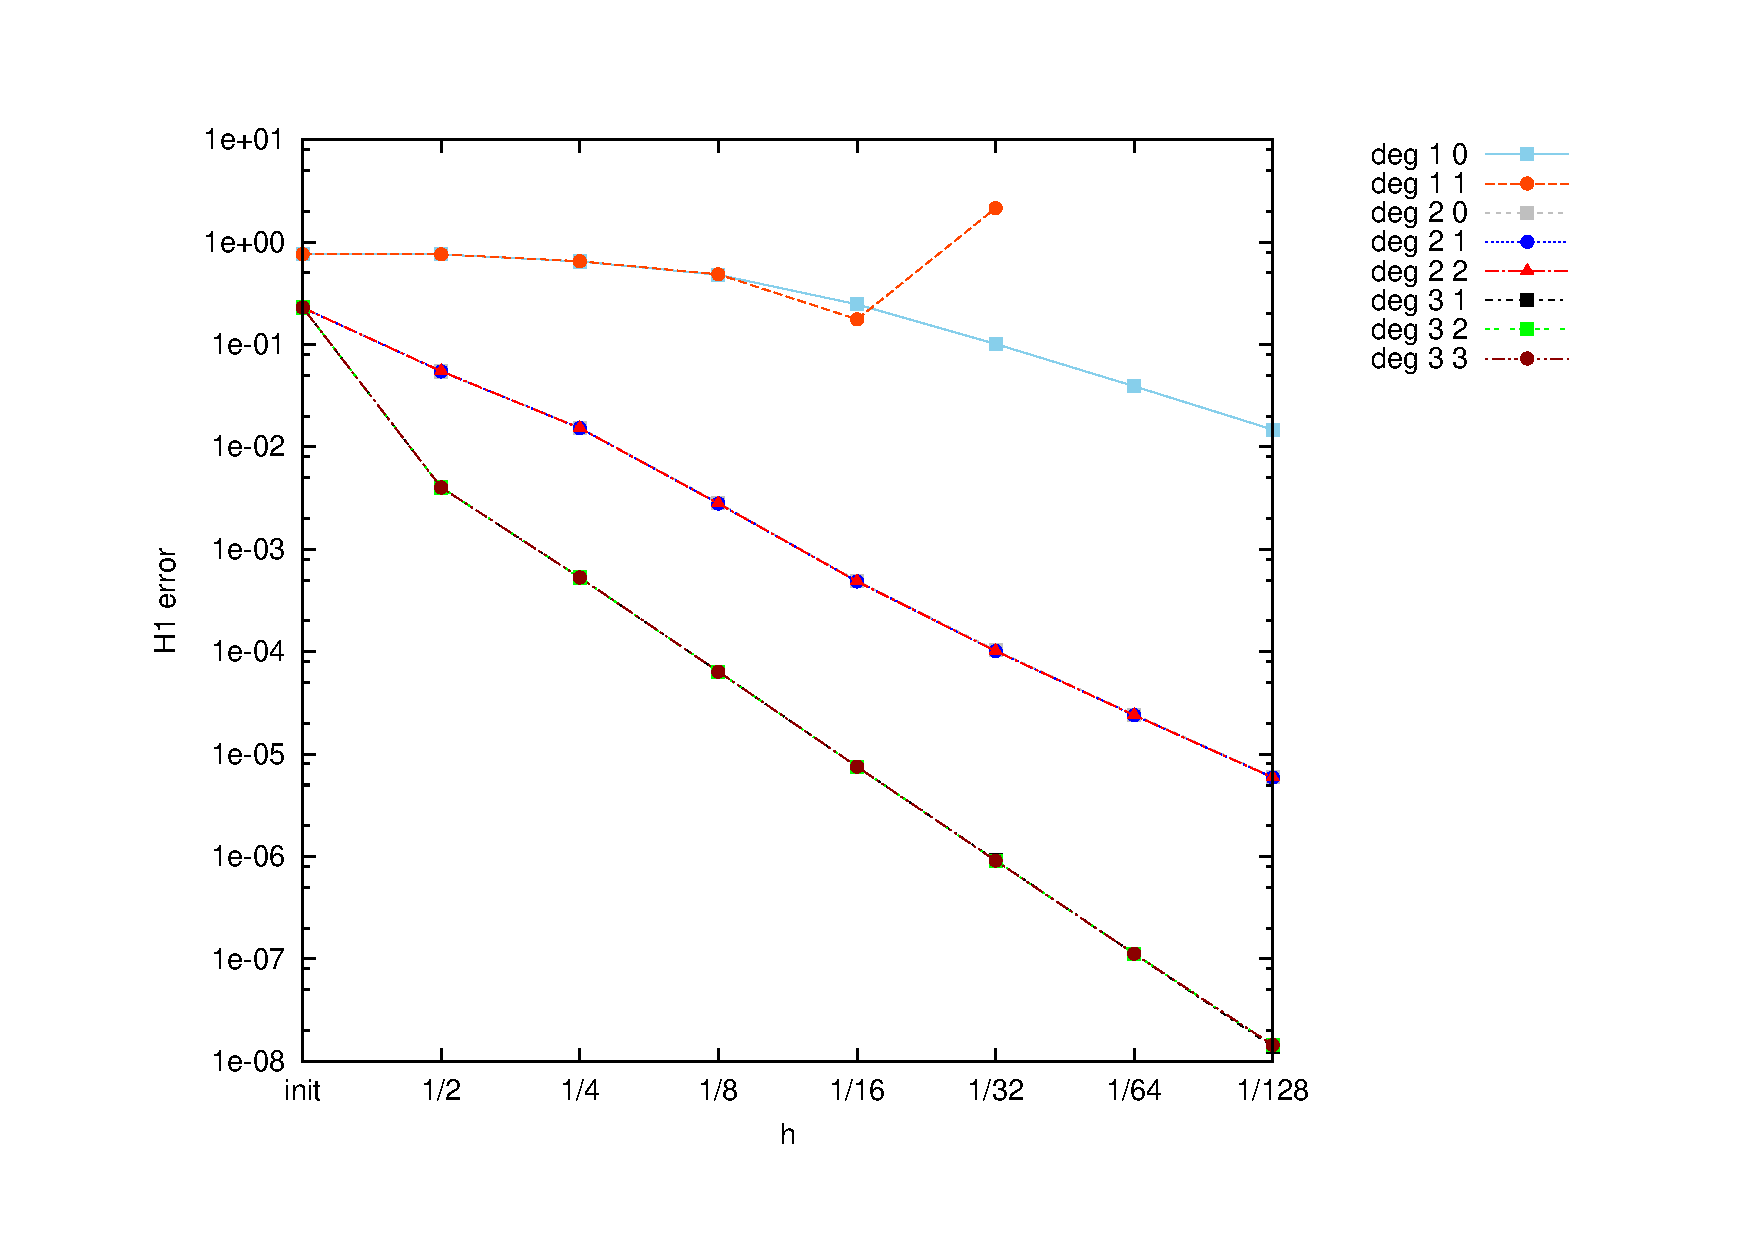
\includegraphics[scale =0.45]{plots/MA1_Neilan_GradJump_h1.pdf}
	\caption{$H^1$ errors for Test \ref{test smooth} and additional gradient jump penalty}
	\label{fig: h1 errors test 1 jump}
\end{figure}

As claimed by Neilan the additional penalisation leads to a convergent method even for low polynomial degrees \cite[Section 5]{Neilan2014}, even in the cases where 1$k_{DH}$ was taken to be small. The only exception is the case $k=1$ and $k_{DH}=1$, for some reason here the method fails. Neilan does not provide any results on this choice of polynomial degrees, he only provides results for the pairs $(k,k_{DH}) \in \{(1,0), (2,2), (3,3)\}$. 

Note that the penalised method performs better than the original ones for higher degrees, too. This is especially visible if $k_{DH}$ was chosen lower than $k$. The numerical orders given in Table \ref{tab: order jump} confirm this observation and we see again that the $L^2$ error decreases with order $k+1$ and the $H^1$ error with the order $k$. We remember that this result was also proven by Neilan (cf. Theorem \ref{thm: error estimate Neilan}, \cite[Theorem 4.2.]{Neilan2014}).

Again the calculated error norms indicate that variation of $k_{DH}$ results only in a slight loss of accuracy. For the cases $k=3$ and $k_{DH} = 2,3$ the errors and hence, in particular the order, are almost equal. 


\begin{table}[H]
\centering
\begin{subtable}[b]{0.45\textwidth}
	\centering
	\pgfplotstabletypeset
	{
		k $k_{DH}$ {numerical order}
		1 0 1.32061
		2 0 2.69871
		2 1 2.93488
		2 2 2.85571
		3 1 3.63116 
		3 2 3.78885
		3 3 3.79348
	}
	\caption{Numerical order in $L^2$ norm}
	\end{subtable}
	\begin{subtable}[b]{0.45\textwidth}
	\centering
	\pgfplotstabletypeset
	{
		k $k_{DH}$ {numerical order}
		1 0 0.978853
		2 0 2.24561
		2 1 2.24836
		2 2 2.24824
		3 1 3.03434
		3 2 3.0286
		3 3 3.02892
	}
	\caption{Numerical order in $H^1$ norm}
	\end{subtable}
	\caption{Numerical order with jump penalty in Test \ref{test smooth}}
\label{tab: order jump}
\end{table}
